\section{Experiments}
This section provides the detailed description of the datasets used to test the implemented methods together with a comparison between the performance achieved by the different models. We provide all the configuration tested and the listing of the values of different parameters in order to allow the reproducibility of the performed tests. We conclude each section showing the achieved results for all the models, comparing them to the expected ones.

In \textbf{\S\ref{sec:data}} we describe the general structure of each dataset, the main characteristics and the pre-processing operations we performed before executing the tests. We used a standardized approach for all the performed test, in particular we implemented the NN in such a way to be compatible with the \texttt{GridSearchCV} model selection class provided by the \texttt{sklearn} library. Following the same approach adopted in the \textit{ML} course, we selected the best model by performing a \textit{k-fold cross validation} by holding out, at each iteration, \textit{20\%} of the data, resulting in a \textit{5-fold cross validation}. The best model selected in this way is the one used in the different tests for comparison. This allowed us to discriminate between different models without the need to manually fine-tune the different hyperparameters of the different models. However, since the main goal of this project is not the one of selecting the best model on the out-of-sample data, we only used the results obtained in the first gridsearch approach to better understand which were the models that better suited our needs. We also notice, as a confirmation of the goodness of the approach and the basic implementation of our models, that the achieved results are in line with the ones we achieved during the \textit{ML} competition.

All the tests were performed on a \texttt{AMD Ryzen 7 Pro 4750u} with 8 physical cores and 16 threads, with a base clock of 1.7GHz.

\input{chapters/experiments/dataset}
\subsection{Model selection}
All the models used for the performance evaluation and comparison were selected following a gridsearch cross-validation schema, specifically a 5-fold cross validation for the \textbf{CUP} dataset and a \textit{StratifiedKFold} cross validation schema for the \textbf{MONK}s datasets. In this paragraph we show the range of tested hyper-parameters used in order to select the best model for each dataset.

\begin{table}[H]
    \begin{center}
    \begin{tabular}{|P{2.cm}||c|c|c|c|c|}
         \hline
         \textbf{Task} & \textbf{batch\_size} & $\boldsymbol{\epsilon}$ & $\boldsymbol{\mu}$ & $\boldsymbol{\lambda}$ & \textbf{sizes} \\ [0.5ex] 
         \hline\hline
         MONK & \{10, 32, None\} & [0.01, 0.1] & [0, 0.9] & [0, 0.1] & \{2, 3, 5\}\\
         \hline
         CUP & \{32, None\} & [0.01, 0.1] & [0, 0.9] & [0, 0.01] & [16, 50]\\
         \hline
    \end{tabular}
    \subcaption{\texttt{SGD} gridsearch ranges.}
    \label{tab:gridSGD}
    \end{center}
    \hspace{2em}
    \begin{center}
    \begin{tabular}{|P{2.cm}||c|c|c|c|}
         \hline
         \textbf{Task} & \textbf{batch\_size} & $\boldsymbol{\epsilon}$  & $\boldsymbol{\lambda}$ & \textbf{sizes} \\ [0.5ex] 
         \hline\hline
         MONK & \{10, 32, None\} & [0.01, 0.1] & [0, 0.1] & \{2, 3, 5\}\\
         \hline
         CUP & \{32, None\} & [0.01, 0.1] & [0, 0.01] & [16, 50]\\
         \hline
    \end{tabular}
    \subcaption{\texttt{SGM} gridsearch ranges.}
    \label{tab:gridSGM}
    \end{center}
    \caption{Gridsearch ranges for both SGD (a) and SGM (b) over \textbf{MONK} and \textbf{CUP} datasets. The search was performed imposing as stopping condition, for both optimizers, a number of epochs equal to \textbf{1000} and a precision computed as norm of the gradient of $\mathbf{1\mathrm{\mathbf{e}}{-4}}$. \textit{Note: the sizes specified in both \textbf{(a)} and \textbf{(b)}, for the CUP row, refers to the amount of units used in \textbf{each} of the hidden layers of the tested network.}}
    \label{tab:grids}
\end{table}
The best models resulting from the searches specified in \hyperref[tab:grids]{\textbf{Table \ref{tab:grids}}} where used to perform the comparisons in \textbf{\S\ref{sec:res}}. \texttt{SGD} models are tested also with the \textit{NAG} variant, as described in \textbf{\hyperref[eq:nag]{Eq. \ref{eq:nag}}}.
\subsection{Results}
\label{sec:res}
In this section we show, for each implemented model, the achieved results and we compare them with the expected ones. We also show a comparison with the two models \textbf{(M1)} and \textbf{(M2)} on the \textbf{CUP} dataset.

For each tested model, we consider the achieved gradient norm and the score in terms of \textit{MSE} as performance metrics. For all the models based on a NN implementation, we imposed a different stopping condition for the two datasets, in particular:
\begin{itemize}
    \item \textbf{MONK}: stopping condition only based on the norm of the gradient, without selecting a particular amount of epochs;
    \item \textbf{CUP}: stopping condition based also on the number of epochs, this was due to the fact that a given accuracy on the norm of the gradient can't be reached by all the used models.
\end{itemize}

\subsubsection{MONK}
In this section we show the comparison of the different models over the three \textbf{MONK} datasets. In particular we compare the achieved losses and gradient, considering the number of epochs and the amount of time necessary to achieve the desired precision.

\begin{figure}[H]
	\centering
	\begin{subfigure}{.45\textwidth}
	    \centering
	    \subcaptionbox{}{%
            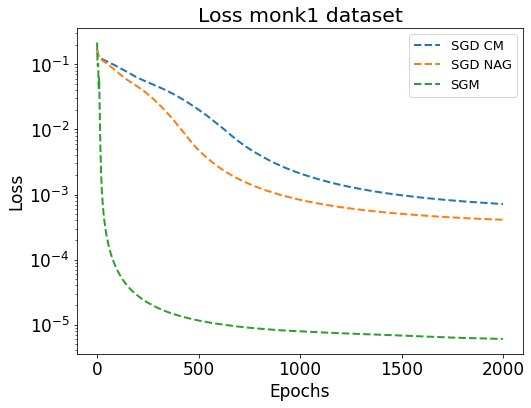
\includegraphics[width=\linewidth]{res/loss_monk1_ep.png}\hspace*{2.5em}%
        }
	\end{subfigure}
	\begin{subfigure}{.45\textwidth}
	    \centering
	    \subcaptionbox{}{%
            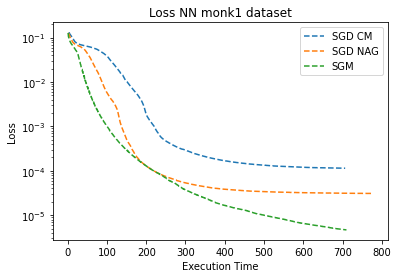
\includegraphics[width=\linewidth]{res/loss_monk1_time.png}\hspace*{2.5em}%
        }
	\end{subfigure}
    \par\bigskip % force a bit of vertical whitespace
	\begin{subfigure}{.45\textwidth}
	    \centering
	    \subcaptionbox{}{%
            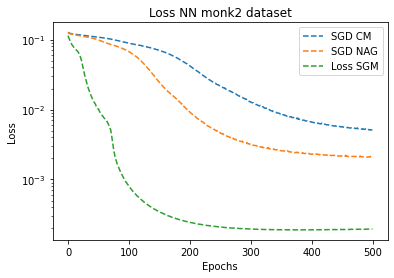
\includegraphics[width=\linewidth]{res/loss_monk2_ep.png}\hspace*{2.5em}%
        }
	\end{subfigure}
	\begin{subfigure}{.45\textwidth}
	    \centering
	    \subcaptionbox{}{%
            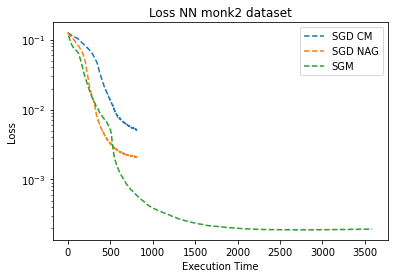
\includegraphics[width=\linewidth]{res/loss_monk2_time.png}\hspace*{2.5em}%
        }
	\end{subfigure}
	\par\bigskip % force a bit of vertical whitespace
	\begin{subfigure}{.45\textwidth}
	    \centering
	    \subcaptionbox{}{%
            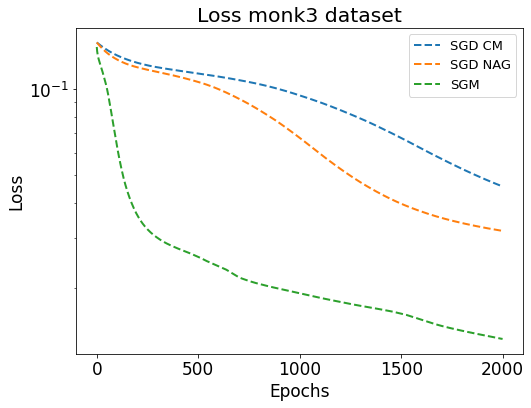
\includegraphics[width=\linewidth]{res/loss_monk3_ep.png}\hspace*{2.5em}%
        }
	\end{subfigure}
	\begin{subfigure}{.45\textwidth}
	    \centering
	    \subcaptionbox{}{%
            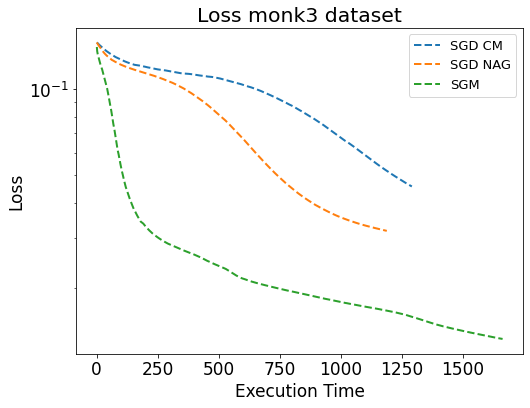
\includegraphics[width=\linewidth]{res/loss_monk3_time.png}\hspace*{2.5em}%
        }
	\end{subfigure}
	\caption{Comparison between the three tested models \texttt{SGD} (both with \textit{CM} and \textit{NAG}) and \texttt{SGM}. On each row we show the comparison on a different \textbf{MONK} dataset and the two columns represent, from left to right, the loss w.r.t.\ the number of epochs and the required time in milliseconds.}
	\label{fig:monk_loss}
\end{figure}

\begin{figure}[H]
	\centering
	\begin{subfigure}{.4\textwidth}
	    \centering
	    \subcaptionbox{}{%
            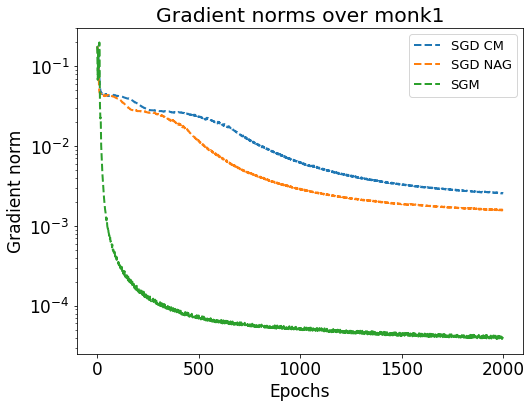
\includegraphics[width=\linewidth]{res/grad_monk1.png}\hspace*{2.5em}%
        }
	\end{subfigure}
	\begin{subfigure}{.4\textwidth}
	    \centering
	    \subcaptionbox{}{%
            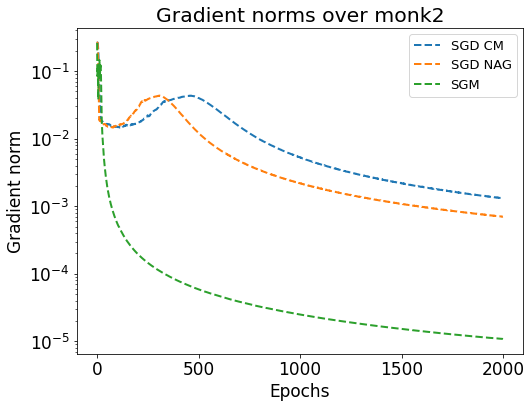
\includegraphics[width=\linewidth]{res/grad_monk2.png}\hspace*{2.5em}%
        }
	\end{subfigure}
	\begin{subfigure}{.45\textwidth}
        \centering
	    \subcaptionbox{}{%
            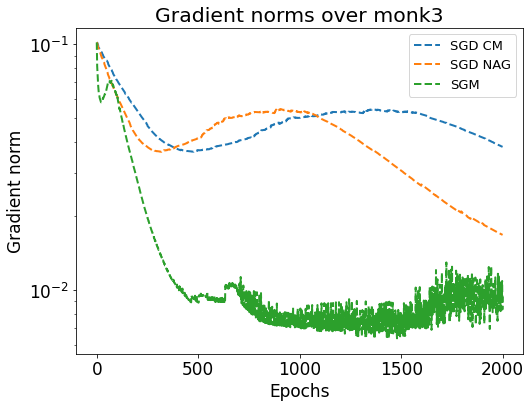
\includegraphics[width=\linewidth]{res/grad_monk3.png}\hspace*{2.5em}%
        }
	\end{subfigure}
	
	\caption{Gradient norm comparison over the three \textbf{MONK} datasets for the three tested models.}
	\label{fig:monk_grad}
\end{figure}

\begin{table}[H]
    \begin{center}
    \begin{adjustwidth}{0.cm}{}
    \begin{center}
    \resizebox{0.9\textwidth}{!}{%
    \begin{tabular}{|P{2.cm}||c|c|c|c|c|c|c|c|}
         \hline
         \textbf{Task} & \textbf{optimizer} & \textbf{batch\_size} & $\boldsymbol{\epsilon}$ & $\boldsymbol{\mu}$ & $\boldsymbol{\lambda}$ & \textbf{sizes} & $\nabla f_*$ & $f_*$ \\ [0.5ex] 
         \hline\hline
         MONK1 & CM & 32 & 0.1 & 0.9 & 0.1 & 5 & \num{1.271e-2} & \num{1.145e-4}\\
         \hline
         MONK1 & NAG & 32 & 0.1 & 0.9 & 0.01] & 5 & \num{6.801e-3} & \num{3.088e-5}\\
         \hline
         MONK1 & SGM & None & 0.1 & - & 0.01 & 5 & \num{8.020e-4} & \num{4.662e-6}\\
         \hline\hline
         MONK2 & CM & 32 & 0.1 & 0.5 & 0.01 & 3 & \num{5.328e-2} & \num{5.079e-3}\\
         \hline
         MONK2 & NAG & 32 & 0.1 & 0.5 & 0.01 & 3 & \num{4.719e-2} & \num{2.090e-3}\\
         \hline
         MONK2 & SGM & 10 & 0.1 & - & 0.01 & 3 & \num{1.935e-2} & \num{1.898e-4}\\
         \hline\hline
         MONK3 & CM & 10 & 0.1 & 0.9 & 0.01 & 5 & \num{1.635e-2} & \num{8.945e-3}\\
         \hline
         MONK3 & NAG & 10 & 0.1 & 0.9 & 0.01 & 5 & \num{7.106e-3} & \num{3.391e-3}\\
         \hline
         MONK3 & SGM & None & 0.1 & - & 0.01 & 5 & \num{2.449e-3} & \num{6.921e-4}\\
         \hline
    \end{tabular}}
    \end{center}
    \end{adjustwidth}
    \subcaption{Test results over \textbf{MONK} datasets. Models chosen via gridsearch as shown in \S\ref{sec:res}}
    \label{tab:res_MONK}
    \end{center}
    \hspace{2em}
    \begin{center}
    \resizebox{0.6\textwidth}{!}{%
    \begin{tabular}{|P{2.cm}||c|c|c|c|c|}
         \hline
         \textbf{Task} & \textbf{optimizer} & \textbf{epochs} & \textbf{total} & \textbf{BP} & \textbf{EP} \\ [0.5ex] 
         \hline\hline
         MONK1 & CM & 500 & 601.93 & 0.078 & 1.203 \\
         \hline
         MONK1 & NAG & 500 & 497.99 & 0.061 & 0.995 \\
         \hline
         MONK1 & SGM & 1000 & 604.02 & 0.228 & 0.604 \\
         \hline\hline
         MONK2 & CM & 500 & 693.86 & 0.062 & 1.387 \\
         \hline
         MONK2 & NAG & 500 & 924.36 & 0.078 & 1.848 \\
         \hline
         MONK2 & SGM & 500 & 3496.17 & 0.210 & 6.992 \\
         \hline\hline
         MONK3 & CM & 500 & 1360.03 & 0.059 & 2.720 \\
         \hline
         MONK3 & NAG & 500 & 1772.94 & 0.074 & 3.545 \\
         \hline
         MONK3 & SGM & 1000 & 751.25 & 0.277 & 0.751 \\
         \hline
    \end{tabular}}
    \subcaption{Execution statistics relative to the models used for testing in table \ref{tab:res_MONK}.}
    \label{tab:gridSGM}
    \end{center}
    \caption{Execution results and performances for the models selected via gridsearch.}
    \label{tab:stat_MONK}
\end{table}

In \hyperref[tab:res_MONK]{\textbf{Table \ref{tab:res_MONK}}} we clearly see an increased cost for the \textit{backpropagation} computation for the \texttt{SGM} model. This was due to the fact that this model requires to update the stepsize at the end of each iteration in order to converge to a solution. This inevitably introduces a bottleneck in the computation of the backpropagation algorithm compared to the \texttt{SGD} model.

\subsubsection{CUP}
In this section we show the comparison of different models over the CUP dataset. We show the achieved loss and gradient norms for all the tested models.
\begin{figure}[H]
	\centering
	\begin{subfigure}{.4\textwidth}
	    \centering
	    \subcaptionbox{}{%
            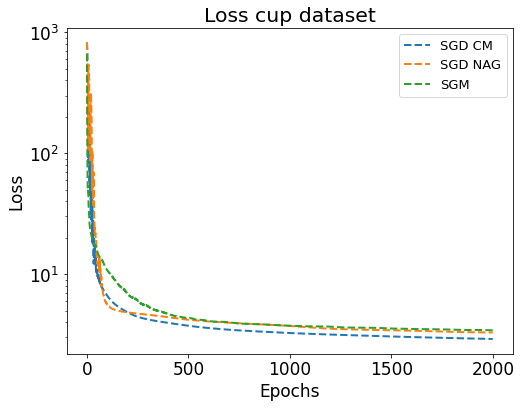
\includegraphics[width=\linewidth]{res/loss_cup_ep.png}\hspace*{2.5em}%
        }
	\end{subfigure}
	\begin{subfigure}{.4\textwidth}
	    \centering
	    \subcaptionbox{}{%
            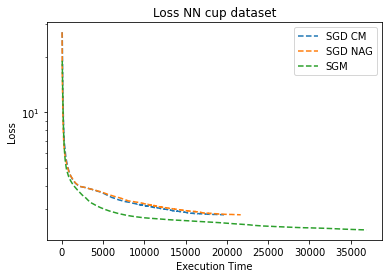
\includegraphics[width=\linewidth]{res/loss_cup_time.png}\hspace*{2.5em}%
        }
	\end{subfigure}
    
	\caption{Comparison between the three tested models \texttt{SGD} (both with \textit{CM} and \textit{NAG}) and \texttt{SGM} over the CUP dataset. Image \textbf{(a)} and \textbf{(b)} show, respectively, the loss w.r.t.\ the number of epochs and the required time in milliseconds.}
	\label{fig:cup_loss}
\end{figure}

\begin{figure}[H]
	\centering
    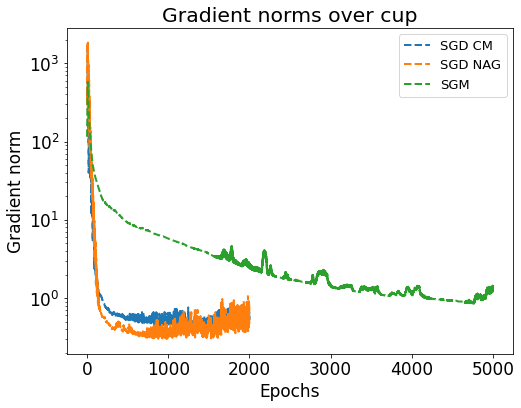
\includegraphics[width=0.4\linewidth]{res/grad_cup.png}\hspace*{2.5em}%
	
	\caption{Gradient norm comparison over the \textbf{CUP} dataset for the three tested models.}
	\label{fig:cup_grad}
\end{figure}

\begin{table}[H]
    \begin{center}
    \begin{adjustwidth}{0.cm}{}
    \begin{center}
    \resizebox{0.9\textwidth}{!}{%
    \begin{tabular}{|P{2.cm}||c|c|c|c|c|c|c|c|}
         \hline
         \textbf{Task} & \textbf{optimizer} & \textbf{batch\_size} & $\boldsymbol{\epsilon}$ & $\boldsymbol{\mu}$ & $\boldsymbol{\lambda}$ & \textbf{sizes} & $\nabla f_*$ & $f_*$ \\ [0.5ex] 
         \hline\hline
         CUP & CM & 32 & 0.1 & 0.9 & 0.1 & 5 & \num{1.271e-2} & \num{1.145e-4}\\
         \hline
         CUP & NAG & 32 & 0.1 & 0.9 & 0.01] & 5 & \num{6.801e-3} & \num{3.088e-5}\\
         \hline
         CUP & SGM & None & 0.1 & - & 0.01 & 5 & \num{8.020e-4} & \num{4.662e-6}\\
         \hline
    \end{tabular}}
    \end{center}
    \end{adjustwidth}
    \subcaption{Test results over \textbf{CUP} dataset. Models chosen via gridsearch as shown in \S\ref{sec:res}}
    \label{tab:res_CUP}
    \end{center}
    \hspace{2em}
    \begin{center}
    \resizebox{0.65\textwidth}{!}{%
    \begin{tabular}{|P{2.cm}||c|c|c|c|c|}
         \hline
         \textbf{Task} & \textbf{optimizer} & \textbf{iterations} & \textbf{total} & \textbf{BP} & \textbf{EP} \\ [0.5ex] 
         \hline\hline
         CUP & CM & 1000 & 20059 & 0.187 & 20.059 \\
         \hline
         CUP & NAG & 1000 & 20061 & 0.182 & 20.061 \\
         \hline
         CUP & SGM & 1000 & 33282 & 0.526 & 33.282 \\
         \hline
    \end{tabular}}
    \subcaption{Execution statistics relative to the models used for testing in table \ref{tab:res_MONK}.}
    \label{tab:gridSGM}
    \end{center}
    \caption{Execution results and performances for the models selected via gridsearch.}
    \label{tab:stat_CUP}
\end{table}
\subsection{Direct Solver}
In this section we show the main results obtained with the implemented direct solver and we compare them with the ones from the out-of-the-box solver from \texttt{Numpy} library. As we show in the following paragraphs, our solver is able to achieve the expected precision and the achieved results are comparable with the ones obtained with the \texttt{Numpy} ones. However, we can't compare our solver to the \texttt{Numpy} one under an execution efficiency standpoint, since our solver lacks all the necessary optimizations needed to achieve the same performances as the library we used to compare our model with.

\subsubsection{QR implementation comparison}
In this section we show the comparison between the implemented algorithm \textbf{(A3)}, needed as an intermediate step for the \textit{LS} solution as specified in \S\ref{sec:qr}, and the \texttt{Numpy} out-of-the-box solver for the \textit{QR} computation.

\begin{figure}[H]
	\centering
	\begin{subfigure}{.45\textwidth}
	    \centering
	    \subcaptionbox{\label{img:a3_qr}}{%
            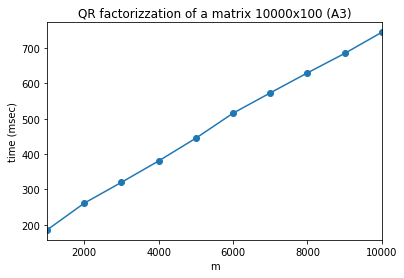
\includegraphics[width=\linewidth]{res/a3_scaling.png}\hspace*{1.5em}%
        }
	\end{subfigure}
	\begin{subfigure}{.45\textwidth}
	    \centering
	    \subcaptionbox{\label{img:np_qr}}{%
            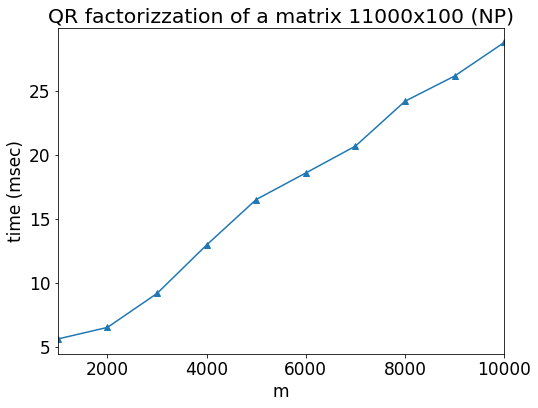
\includegraphics[width=\linewidth]{res/np_scaling.png}\hspace*{1.5em}%
        }
	\end{subfigure}
	
	\begin{subfigure}{.45\textwidth}
	    \centering
	    \subcaptionbox{\label{img:scaling}}{%
            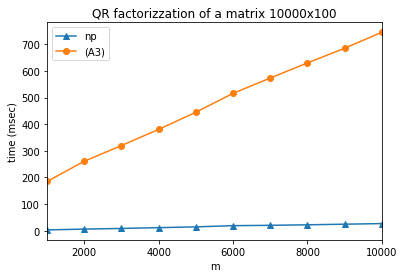
\includegraphics[width=\linewidth]{res/scaling_comp.png}\hspace*{1.5em}%
        }
	\end{subfigure}
    
	\caption{Comparison between the implemented \textbf{(A3)} algorithm with the \texttt{Numpy} off-the-shelf-solver. In figure \textbf{\ref{img:a3_qr}} and \textbf{\ref{img:np_qr}} there are, respectively, the performances in QR computation for the implemented \textbf{(A3)} solver and the \texttt{Numpy} one over datasets with increasing dimensions, up to 10000x100. In \textbf{\ref{img:scaling}} the same plots are put together to highlight the difference in performance.}
	\label{fig:scaling_qr}
\end{figure}

\vspace*{-1cm}
\begin{table}[H]
    \begin{center}
    \begin{adjustwidth}{0.cm}{}
    \begin{center}
    \resizebox{0.65\textwidth}{!}{%
    \begin{tabular}{|P{2.cm}||c|c|c|c|}
        \hline
         \textbf{m} & \textbf{time (A3)} & \textbf{delta (A3)} & \textbf{time (NP)} & \textbf{delta (NP)}\\ [0.5ex]
         \hline\hline
        1000 & 185.1129 & - & 3.1858 & -\\\hline
        2000 & 260.9890 & 75.8761 & 6.3108 & 3.1250\\\hline
        3000 & 319.9584 & 58.9694 & 8.6793 & 2.3686\\\hline
        4000 & 380.6262 & 60.6678 & 11.6935 & 3.0141\\\hline
        5000 & 444.9249 & 64.2987 & 14.6366 & 2.9432\\\hline
        6000 & 515.8109 & 70.8860 & 19.1323 & 4.4956\\\hline
        7000 & 573.2926 & 57.4817 & 20.4345 & 1.3022\\\hline
        8000 & 630.0169 & 56.7243 & 22.3729 & 1.9384\\\hline
        9000 & 685.0543 & 55.0375 & 24.7365 & 2.3636\\\hline
        10000 & 745.0878 & 60.0335 & 26.9332 & 2.1967\\\hline
    \end{tabular}}
    \end{center}
    \end{adjustwidth}
    \caption{Scaling performances of the implemented algorithm \textbf{(A3)} and the \texttt{Numpy} one. Time is expressed in milliseconds.}
    \label{tab:scaling_perf_qr}
    \end{center}
\end{table}
As we can see in both \hyperref[fig:scaling_qr]{\textbf{Figure \ref{fig:scaling_qr}}} and \hyperref[tab:scaling_perf]{\textbf{Table \ref{tab:scaling_perf_qr}}}, the implemented algorithm for \textit{QR} computation scales linearly with the \textbf{m} dimension of the matrix, as expected theoretically and as shown at the end of  \textbf{\S\ref{sec:ls_scaling}} paragraph. However, given that our algorithm does not make use of extensive optimizations, this reflects on the completion time required for the computation of the \textit{QR} factorization.

\subsubsection{LS implementation comparison}
In this paragraph we show the comparison between the implemented algorithm \textbf{(A3)} and the \texttt{Numpy} solver. We used a sequence of randomly generated matrix with increasing dimension \textit{m} in [1000, 10000], in order to highlight the scaling performances and show that they are in line with the theoretically expected ones. We decided to fix the \textit{n} dimension to 100 in order to allow the algorithm to terminate in a reasonable amount of time one the machine at our disposal.

\begin{figure}[H]
	\centering
	\begin{subfigure}{.4\textwidth}
	    \centering
	    \subcaptionbox{\label{img:a3_qr}}{%
            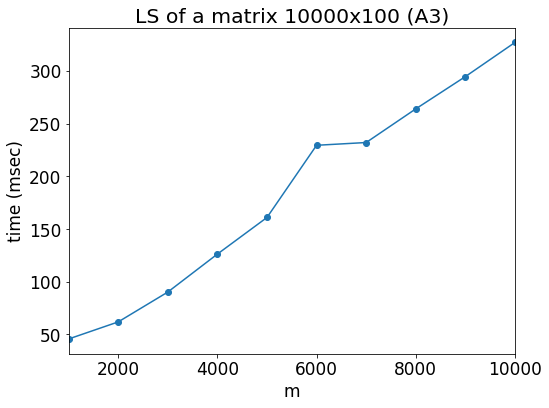
\includegraphics[width=\linewidth]{res/a3_ls_scaling.png}\hspace*{1.5em}%
        }
	\end{subfigure}
	\begin{subfigure}{.4\textwidth}
	    \centering
	    \subcaptionbox{\label{img:np_qr}}{%
            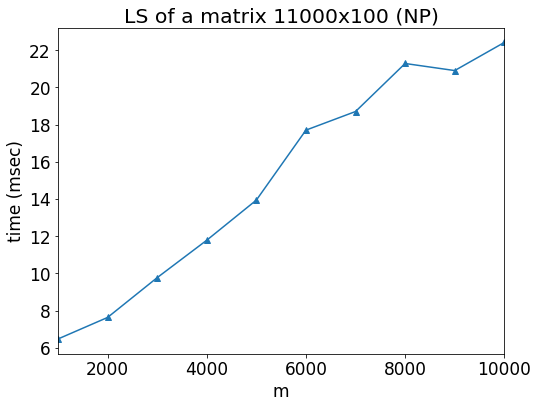
\includegraphics[width=\linewidth]{res/np_ls_scaling.png}\hspace*{1.5em}%
        }
	\end{subfigure}
	
	\begin{subfigure}{.4\textwidth}
	    \centering
	    \subcaptionbox{\label{img:scaling}}{%
            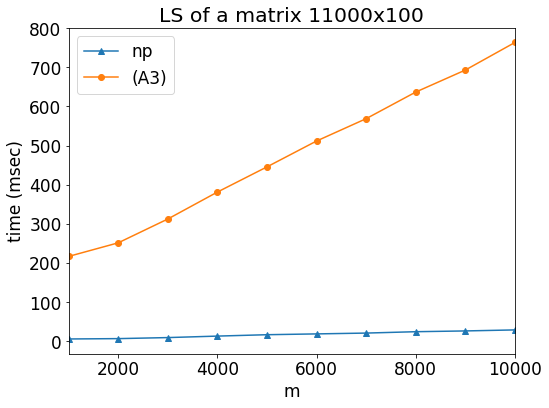
\includegraphics[width=\linewidth]{res/ls_scaling_comp.png}\hspace*{1.5em}%
        }
	\end{subfigure}
    
	\caption{Comparison between the implemented \textbf{(A3)} algorithm with the \texttt{Numpy} off-the-shelf-solver. In figure \textbf{\ref{img:a3_qr}} and \textbf{\ref{img:np_qr}} there are, respectively, the performances in LS computation for the implemented \textbf{(A3)} solver and the \texttt{Numpy} one. In \textbf{\ref{img:scaling}} the same plots are put together to highlight the difference in performance.}
	\label{fig:scaling_ls}
\end{figure}

\begin{table}[H]
    \begin{center}
    \begin{adjustwidth}{0.cm}{}
    \begin{center}
    \begin{tabular}{|P{2.cm}||c|c|c|c|}
        \hline
         \textbf{m} & \textbf{time (A3)} & \textbf{delta (A3)} & \textbf{time (NP)} & \textbf{delta (NP)}\\ [0.5ex]
         \hline\hline
        1000 & 33.2898 & - &    5.4329 & -\\\hline
        2000 & 61.8065 & 28.5167 & 8.0054 & 2.5725\\\hline
        3000 & 98.6733 & 36.8669 & 10.0943 & 2.0889\\\hline
        4000 & 128.8937 & 30.2204 & 11.8025 & 1.7082\\\hline
        5000 & 165.1421 & 36.2484 & 14.2208 & 2.4183\\\hline
        6000 & 208.6527 & 43.5106 & 16.6491 & 2.4283\\\hline
        7000 & 235.6089 & 26.9562 & 18.2518 & 1.6028\\\hline
        8000 & 275.4459 & 39.8371 & 20.8711 & 2.6193\\\hline
        9000 & 310.8279 & 35.3820 & 21.2367 & 0.3656\\\hline
        10000 & 334.9303  & 24.1024 & 22.9452 & 1.7085\\\hline
    \end{tabular}
    \end{center}
    \end{adjustwidth}
    \caption{Scaling performances of the implemented algorithm \textbf{(A3)} and the \texttt{Numpy} one. Time is expressed in milliseconds.}
    \label{tab:scaling_perf_ls}
    \end{center}
\end{table}

We can clearly see, both in \hyperref[fig:scaling_ls]{\textbf{Figure \ref{fig:scaling_ls}}} and \hyperref[tab_scaling_perf_ls]{\textbf{Table \ref{tab:scaling_perf_ls}}}, that the algorithm linearly scale with the \textit{m} dimension, as expected. Once again, the comparison under a computational efficiency standpoint can't be done properly, since our algorithm requires 10 times more with respect to the \texttt{Numpy} one.

Finally, in table \hyperref[tab:cup_res_direct]{\textbf{Table \ref{tab:cup_res_direct}}} we can see the results comparison in the Least Square solution for the CUP dataset by using the implemented solver and the one offered by the \texttt{Numpy} library. We also show the error in the reconstruction of the original matrix via \textit{QR} factorization and we can clearly see the goodness of the implementation with reference to highly optimized solvers.

\begin{table}[H]
    \begin{center}
    \begin{adjustwidth}{-0.4cm}{}
    \begin{center}
    \begin{tabular}{|P{2.cm}||c|c|c|c|}
        \hline
         \textbf{Task} & \textbf{residual (A3)} & \textbf{residual (NP)} & \textbf{QR to A (A3)} & \textbf{QR to A (NP)}\\ [0.5ex]
         \hline\hline
        CUP & 1.0538 & 0.9963 &  4.93339e-16 & 3.28932e-16\\
        \hline
        RANDOM & 1.0047 & 0.9953 & 7.89014e-16 & 3.92280e-16\\
        \hline
    \end{tabular}
    \end{center}
    \end{adjustwidth}
    \caption{Residual and reconstruction relative errors for the \textbf{(A3)} algorithm and the \texttt{Numpy} one.}
    \label{tab:cup_res_direct}
    \end{center}
\end{table}

However, even if the reconstruction error is up to machine precision, we can't state the same for what concerns the residual error for both of the compared algorithms. Since the problems are far from being linear, the solution found by the LS solver we used is very poor and it is close to the one achieved on a random dataset generated with a gaussian distribution.

As a final test, we checked if the precision in the results was maintaining at a stable and reasonable level also for bigger matrices. In \hyperref[tab:scaling_huge]{\textbf{Table \ref{tab:scaling_huge}}} we show the relative errors of the residual and the reconstruction error for datasets with the \textit{m} dimension in [10000, 50000] with scaling factor of 10000 while keeping the \textit{n} dimension once again fixed to 100.

\begin{table}[H]
    \begin{center}
    \begin{adjustwidth}{0.cm}{}
    \begin{center}
    \begin{tabular}{|P{2.cm}||c|c|c|c|}
        \hline
         \textbf{m} & \textbf{residual (A3)} & \textbf{residual (NP)} & \textbf{QR to A (A3)} & \textbf{QR to A (NP)}\\ [0.5ex]
         \hline\hline
        10000 & 1.004136 & 0.995936 & 1.148071e-15 & 5.144102e-16\\\hline
        20000 & 1.001552 & 0.997711 & 7.093753e-16 & 5.028219e-16\\\hline
        30000 & 1.001714 & 0.998399 & 6.781397e-16 & 4.979521e-16\\\hline
        40000 & 1.001585 & 0.998724 & 7.984209e-16 & 4.945500e-16\\\hline
        50000 & 1.001005 & 0.999045 & 8.001721e-16 & 4.950132e-16\\\hline
    \end{tabular}
    \end{center}
    \end{adjustwidth}
    \caption{Scaling performances of the implemented algorithm \textbf{(A3)} and the \texttt{Numpy} one.}
    \label{tab:scaling_huge}
    \end{center}
\end{table}

As we can see, also for this kind of test, the implemented algorithm attains a similar precision to the one provided by the \texttt{Numpy} library.

